% Created 2021-09-27 Mon 12:00
% Intended LaTeX compiler: xelatex
\documentclass[letterpaper]{article}
\usepackage{graphicx}
\usepackage{grffile}
\usepackage{longtable}
\usepackage{wrapfig}
\usepackage{rotating}
\usepackage[normalem]{ulem}
\usepackage{amsmath}
\usepackage{textcomp}
\usepackage{amssymb}
\usepackage{capt-of}
\usepackage{hyperref}
\setlength{\parindent}{0pt}
\usepackage[margin=1in]{geometry}
\usepackage{fontspec}
\usepackage{svg}
\usepackage{cancel}
\usepackage{indentfirst}
\setmainfont[ItalicFont = LiberationSans-Italic, BoldFont = LiberationSans-Bold, BoldItalicFont = LiberationSans-BoldItalic]{LiberationSans}
\newfontfamily\NHLight[ItalicFont = LiberationSansNarrow-Italic, BoldFont       = LiberationSansNarrow-Bold, BoldItalicFont = LiberationSansNarrow-BoldItalic]{LiberationSansNarrow}
\newcommand\textrmlf[1]{{\NHLight#1}}
\newcommand\textitlf[1]{{\NHLight\itshape#1}}
\let\textbflf\textrm
\newcommand\textulf[1]{{\NHLight\bfseries#1}}
\newcommand\textuitlf[1]{{\NHLight\bfseries\itshape#1}}
\usepackage{fancyhdr}
\pagestyle{fancy}
\usepackage{titlesec}
\usepackage{titling}
\makeatletter
\lhead{\textbf{\@title}}
\makeatother
\rhead{\textrmlf{Compiled} \today}
\lfoot{\theauthor\ \textbullet \ \textbf{2021-2022}}
\cfoot{}
\rfoot{\textrmlf{Page} \thepage}
\renewcommand{\tableofcontents}{}
\titleformat{\section} {\Large} {\textrmlf{\thesection} {|}} {0.3em} {\textbf}
\titleformat{\subsection} {\large} {\textrmlf{\thesubsection} {|}} {0.2em} {\textbf}
\titleformat{\subsubsection} {\large} {\textrmlf{\thesubsubsection} {|}} {0.1em} {\textbf}
\setlength{\parskip}{0.45em}
\renewcommand\maketitle{}
\author{Houjun Liu}
\date{\today}
\title{Kennedy Is Frustrating}
\hypersetup{
 pdfauthor={Houjun Liu},
 pdftitle={Kennedy Is Frustrating},
 pdfkeywords={},
 pdfsubject={},
 pdfcreator={Emacs 28.0.50 (Org mode 9.4.4)}, 
 pdflang={English}}
\begin{document}

\tableofcontents



\section{Kennedy Is Frustrating}
\label{sec:orgbec3155}
\begin{figure}[htbp]
\centering
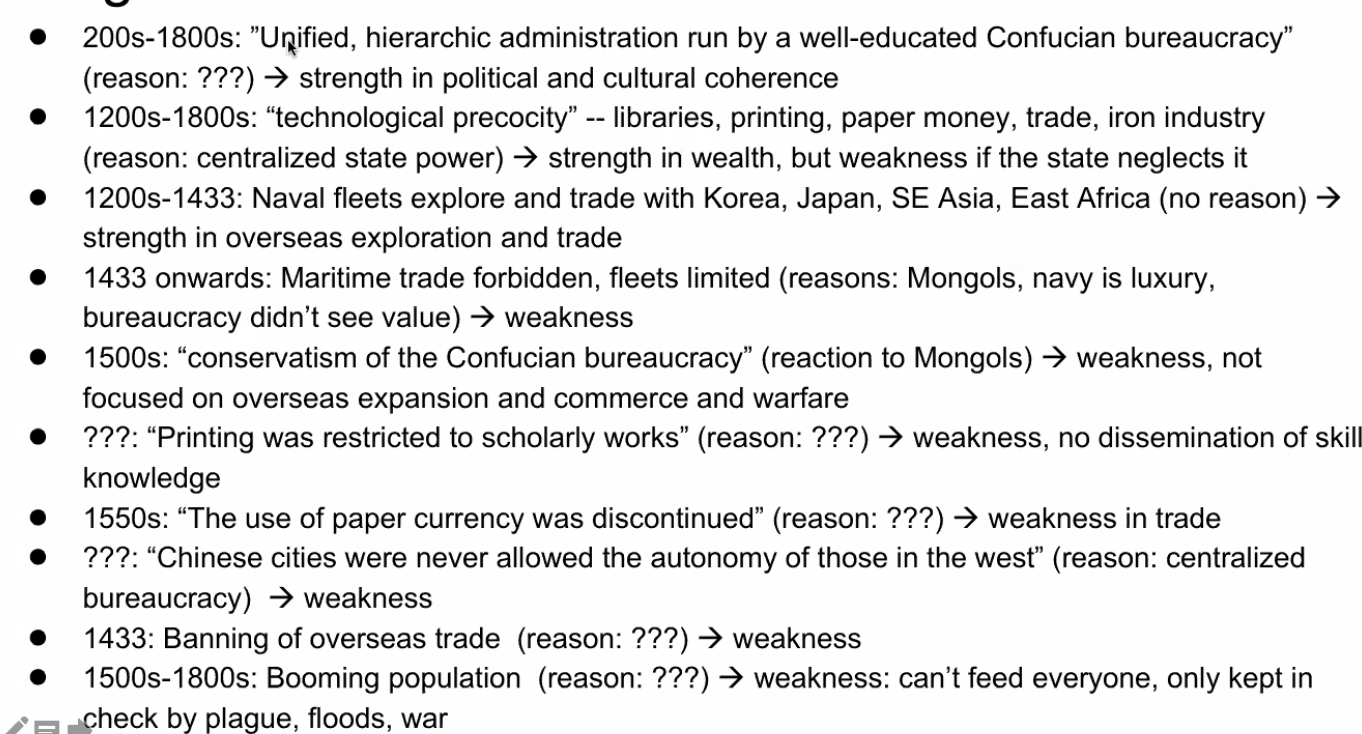
\includegraphics[width=.9\linewidth]{./2020HIST201/Screen Shot 2020-08-31 at 9.30.01 AM.png}
\caption{Screen Shot 2020-08-31 at 9.30.01 AM.png}
\end{figure}

His arguments are not very well supported. For instance, his argument
that orthodox Confucianism stopped trade (and ???, then) decline for
China.

Missing was pieces of evidence could have caused tremendous difficulty.

\begin{quote}
"I don't need arguments to support his claims, I just need to claim
harder" --- Kennedy
\end{quote}

\begin{itemize}
\item "These people failed because they cared about their own people" ---
Both Empires
\item "These people failed because they used a strategy that have worked for
them and is working" --- Ming w.r.t. Confusianism
\item "These people failed because they are too good and managing an empire"
--- Ottomans w.r.t. to the Romanitus
\end{itemize}

\subsection{His Frustrating Arguments}
\label{sec:org6e716a1}
\begin{quote}
One is obliged to stress the words "potential power" because the
evolution of the gunned long-range sailing ship was a slow, often
uneven development\ldots{}. Moreover, there were considerable arguments in
favor of continuing to deploy galleys in the Mediterranean and the
Black Sea; they were swifter on many occasions, more maneuverable\ldots{}
which, for the Turks, outweighed the disadvantages of their being
short-ranged and unable to to act in heavy seas. (25)
\end{quote}

Kennedy's framing of \emph{potential power} is basically saying "Turks, why
did you not see the benefits of this thing that you could not possibly
have seen given the circumstances? Why don't you time travel?"
Development of large maritime ships was slow
\end{document}
